\chapter{Introduction}

For the past decade, numerical weather prediction (NWP) has been the primary approach for weather forecasting. NWP involves the numerical integration of partial differential equations, starting from the best estimate of the current state of the Earth system, to produce a weather forecast. In a standard NWP framework, a weather prediction is obtained through a deductive inference process, where the laws of physics are used to derive a deterministic forecast from the best possible initial conditions. These initial conditions are obtained by optimally combining Earth system observations and short-range forecasts through a process known as \textit{data assimilation}.\\

However, the Earth's state can never be known perfectly, and to account for this, \textit{ensemble forecasting} is often used. This involves making multiple forecasts with small perturbations from a Gaussian distribution around the uncertainties in the system. While NWP has seen significant improvements in recent years, the biggest drawback is still the computational resources required to make accurate predictions in an operational context.\\

Limited area modeling is crucial as it allows for high-resolution forecasts over specific regions without the need to model the entire globe, thereby significantly reducing computational costs. By focusing computational resources on a smaller area, limited area models (LAMs) can provide more detailed and accurate forecasts for local regions, which is essential for applications such as severe weather warnings, local climate studies, and resource management. Additionally, to compute high-resolution forecasts, high-resolution data are required. Currently, the best resolution available for a global forecast is 0.25°.\\

In this context, data-driven modeling based on machine learning (ML) is showing great potential for weather forecasting applications. ML-based models offer the promise of delivering forecasts at a much lower computational cost, along with potential benefits such as increased timeliness and potentially increased accuracy.\\

The aim of this project is to develop a local weather forecasting framework based on machine learning (ML) techniques using historical data from the ERA5 dataset. To achieve this goal, an initial approach will be devised that involves inputting two types of data into our system:\\

\begin{itemize}
    \item The low-resolution state of our system at time \( t + \Delta t \), which can initially be obtained from the ERA5 dataset. In the context of actual forecasting, these data can subsequently be replaced by a global model.
    \item The high-resolution spatial state of our system at times \( t \) and \( t - \Delta t \) over a local range (e.g., 0.25° of latitude by 0.25° of longitude).
\end{itemize}

\vspace{2em}

By utilizing these two types of data, we aim to predict local weather conditions at time \( t + \Delta t \) with higher resolution than the global state and create a proof of concept for a higher resolution forecast for a limited area. To accomplish this, ML techniques will be employed to train our forecasting model using historical data. The performance of our model will then be evaluated using WeatherBench2 \cite{Weatherbench}.


\section{Dataset}

\section{Dataset}

ERA5 is a meteorological and climatological dataset provided by the European Centre for Medium-Range Weather Forecasts (ECMWF). It is a reanalysis dataset that combines model data with observations from around the world to create a globally complete and consistent dataset. ERA5 provides hourly estimates for a wide range of atmospheric, ocean-wave, and land-surface quantities, along with an uncertainty estimate. The dataset is available from 1940 onwards and is updated daily with a delay of approximately five days. 

The data is regridded onto a regular lat-lon grid of 0.25 degrees for reanalysis and 0.5 degrees for uncertainty estimation. The time step between two system states is 1 hour. ERA5 is the primary dataset used by Machine Learning-based Weather Prediction (MLWP) systems.



\section{How do we use the data}

\subsection{Train test validation}

For the period I suggest that we take as KARINA and other model did which is the years 1979 to 2015 for training, 2016 and 2017 are for validation and 2018 as formal test. The choice to take data from 1979 onwards is three fold : first it correspond to the state of the art models choices, secondly it is the most recent years and it has been shown (show citation) that the models output might need the most recent years to make the best forecast and account for global warming trend and third the data before 1979 is said to be less trustworthy at this resolution.\\

\subsection*{For the local model}

We want the regional model to cover an area of 3000 km by 2000 km, which represents approximately 30 degrees by 20 degrees. With a resolution of 0.25 degrees for our data, this corresponds to a grid of approximately 120 by 80. We might choose 37 pressure level as graphCast did for the high resolution state. We will take from 30 to 50 N° and 125 to 155 E°.\\

We will take 66 variables consisting of six surface variables and five variables with 12 vertical pressure levels from the surface to the lower stratosphere, known as prognostic variables of the Earth’s atmosphere. Accordingly with the study of  \cite{cheon2024advancing} we will use the following variables and the orography:\\

\begin{table}[!h]
	\caption{Comprehensive List of Key Atmospheric Variables for Climate Modeling, Corresponding Short Names, Vertical Measurement Levels hPa), and Units.}
	\centering
    \scriptsize
	\begin{tabularx}{\textwidth}{@{}lXXXX@{}}
		\toprule
		Variable name & Short name & Vertical levels (hPa) & Units & \\
		\midrule
		Zonal wind & U & 1000, 925, 850, 800, 700, 600, 500, 400, 300, 200, 100, 50 & m/s & \\
		\addlinespace
		Meridional wind & V & 1000, 925, 850, 800, 700, 600, 500, 400, 300, 200, 100, 50 & m/s & \\
		\addlinespace
		Temperature & T & 1000, 925, 850, 800, 700, 600, 500, 400, 300, 200, 100, 50 & K & \\
		\addlinespace
		Specific humidity & Q & 1000, 925, 850, 800, 700, 600, 500, 400, 300, 200, 100, 50 & kg/kg & \\
		\addlinespace
		Geopotential & Z & 1000, 925, 850, 800, 700, 600, 500, 400, 300, 200, 100, 50 & m\(^2\)/s\(^2\) & \\
		\addlinespace
		2m temperature & T2m & & K & \\
		\addlinespace
		Mean sea level pressure & MSL & & Pa & \\
		\addlinespace
		Surface air pressure & SP & & Pa & \\
		\addlinespace
		Total column vertically-integrated water vapour & TCWV & & kg/m\(^2\) & \\
		\addlinespace
		Skin temperature & SKT & & K & \\
		\addlinespace
		TOA incident solar radiation & TISR & & J/m\(^2\) & \\
		\bottomrule
	\end{tabularx}
	\label{tab:variables}
\end{table}

It seems that we could do it that way but we have to check \href{https://cds.climate.copernicus.eu/cdsapp#!/dataset/reanalysis-era5-complete?tab=form}{here}: \\

For the query of all variables : 
\scriptsize
\begin{Verbatim}
    #!/usr/bin/env python
import cdsapi

c = cdsapi.Client()

c.retrieve("reanalysis-era5-complete", {
    "class": "ea",
    "date": "1979-12-01/to/2015-12-31",
    "expver": "1",
    "levtype": "sfc",
    "param": "134.128/137.128/151.128/165.128/167.128/235.128",  #165.128 TOA incident solar radiation
    "stream": "oper",
    "time": "00:00:00/01:00:00/02:00:00/03:00:00/04:00:00/05:00:00/06:00:00/07:00:00/
    08:00:00/09:00:00/10:00:00/11:00:00/12:00:00/13:00:00/14:00:00/15:00:00/16:00:00/
    17:00:00/18:00:00/19:00:00/20:00:00/21:00:00/22:00:00/23:00:00",
    "type": "an"
}, "output1")

c.retrieve("reanalysis-era5-complete", {
    "class": "ea",
    "date": "1979-12-01/to/2015-12-31",
    "expver": "1",
    "levelist": "50/100/200/300/400/500/600/700/800/850/925/1000",
    "levtype": "pl",
    "param": "129.128/130.128/131/132/133.128"
    "stream": "oper",
    "time": "00:00:00/01:00:00/02:00:00/03:00:00/04:00:00/05:00:00/06:00:00/07:00:00/
    08:00:00/09:00:00/10:00:00/11:00:00/12:00:00/13:00:00/14:00:00/15:00:00/16:00:00/
    17:00:00/18:00:00/19:00:00/20:00:00/21:00:00/22:00:00/23:00:00",
    "type": "an"
}, "output2")

\end{Verbatim}
\normalsize

\section{Model to Develop}

The aim of this internship is to develop a machine learning model that provides as output (\textbf{Y}) a regional-scale, high-resolution weather forecast, which will be referred to as High Resolution Local (\textbf{HRL}) in this document. Initially, the input (\textbf{X}) will be an HRL at time t, denoted as \textbf{HRL(t)}. This first model will represent a simple forecast. Subsequently, a low-resolution global model, referred to as Low Resolution Global (\textbf{LRG}), will be added to the input to potentially improve the system's predictions by providing context.

The work of \href{https://events.ecmwf.int/event/172/contributions/1769/attachments/877/1550/Machine-Learning-WS_Mdini.pdf}{Maha Mdini} should be analyzed to identify any ideas that could be incorporated into the future model.

\vspace{2em}

\begin{tabular}{>{\bfseries}l<{\hspace{1em}} >{\centering\arraybackslash}p{7cm} >{\raggedleft\arraybackslash}p{2cm}}
\hline
\textbf{Model to Develop} & \textbf{Input (X)} & \textbf{Output (Y)}\\
\hline
Model 1 & HRL(t) & HRL(t+dt) \\
Model 2 &  HRL(t) + LRG(t) & HRL(t+dt) \\
Model 3 &  HRL(t) + LRG(t) + LRG (t+dt) & HRL(t+dt) \\
Model 4 & autoregressive & HRL(t+dt) \\
\end{tabular}

\subsection{Model 1: Simple Forecast within a Region}

\begin{figure}[ht]
\centering
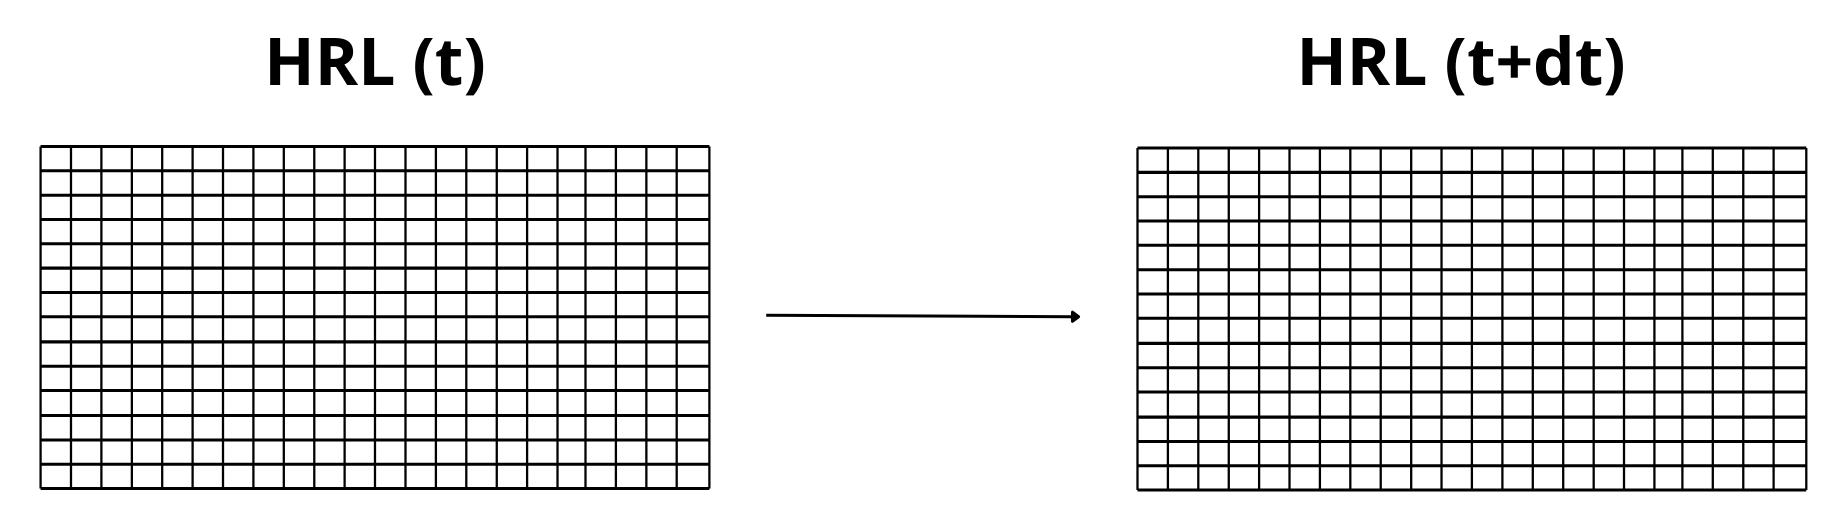
\includegraphics[width=0.9\textwidth]{media/model1.png}
\caption{Architecture of Model 1: Simple Forecast}
\label{fig}
\end{figure}

This model represents a simple forecast within a region with a known state at time t on a fine grid to obtain a known state at time t+dt on a fine grid.

\subsection{Model 2: Forecast with Boundary Conditions}

\begin{figure}[ht]
\centering
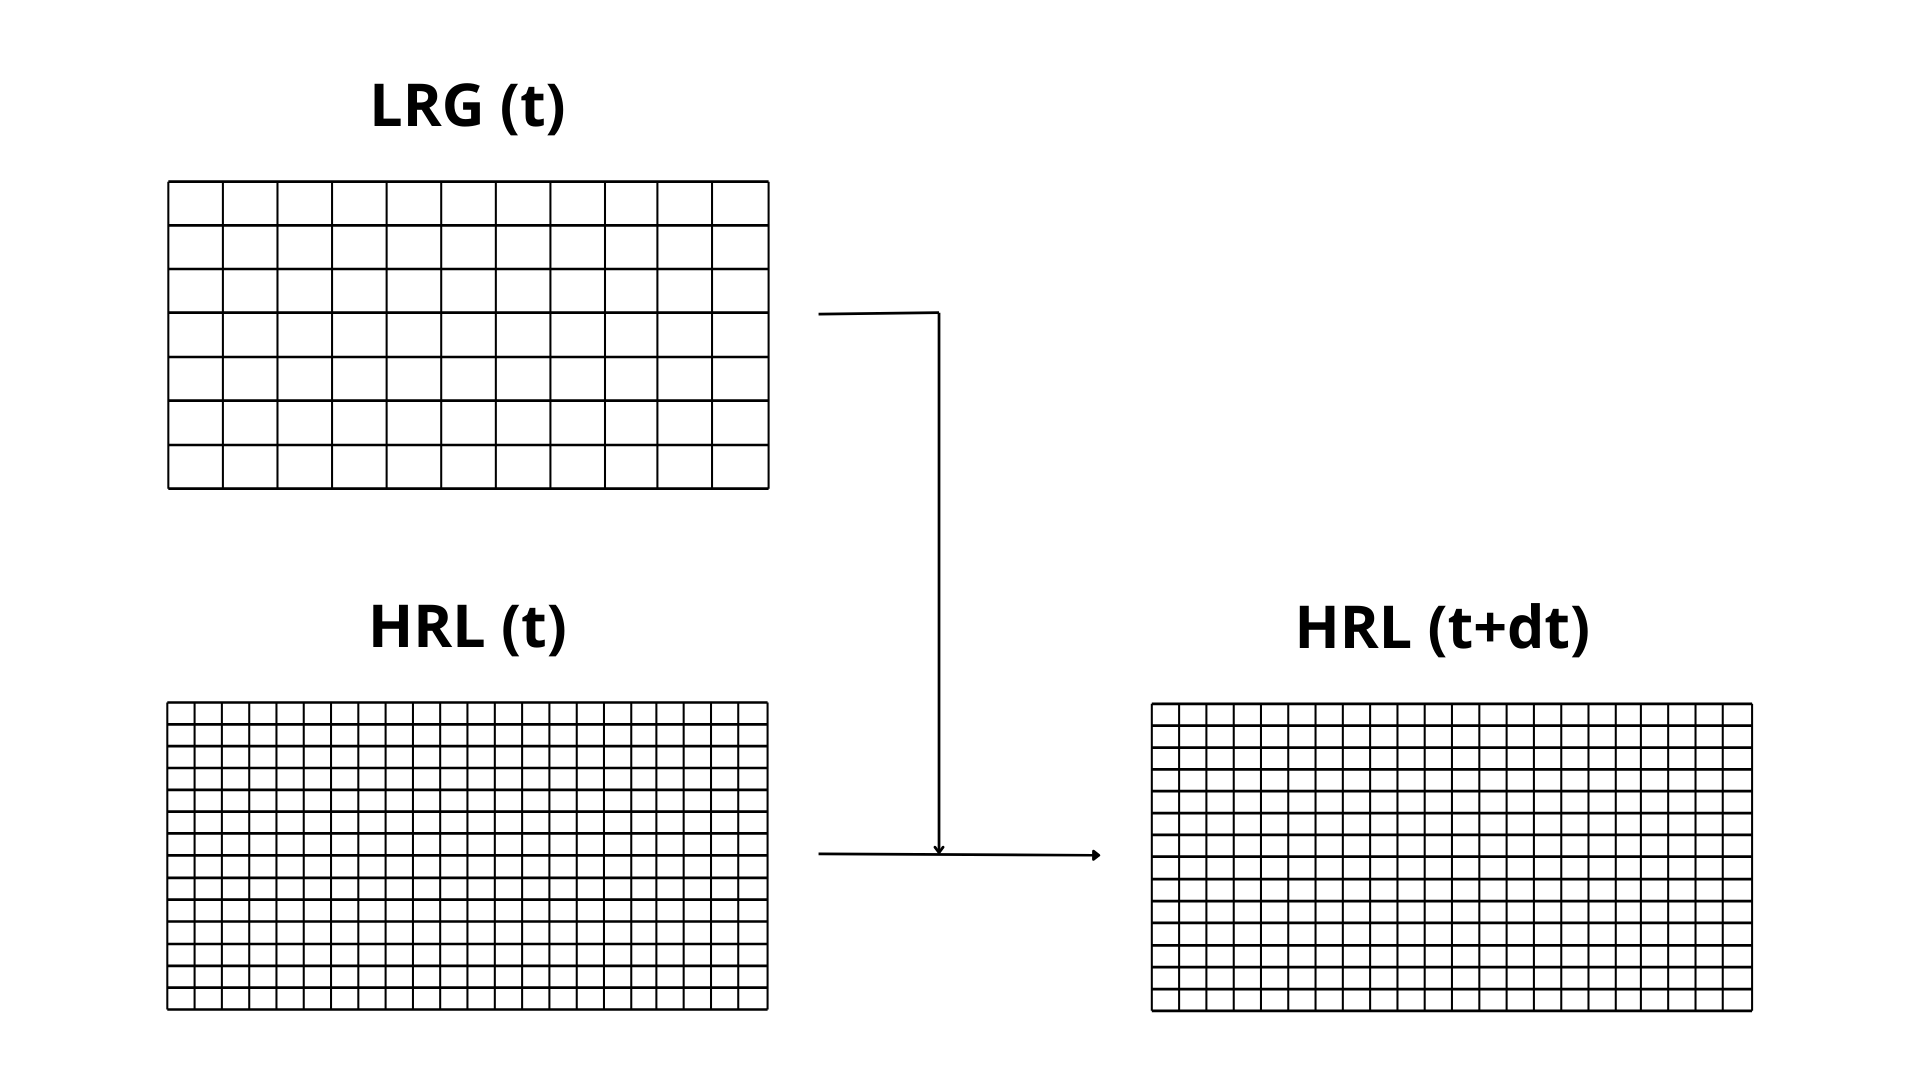
\includegraphics[width=0.9\textwidth]{media/model2.png}
\caption{Architecture of Model 2: Forecast with Degraded Boundary Conditions}
\label{fig}
\end{figure}

The objective of this model is to test whether having a broader system state at time t (boundary conditions) with lower resolution can yield better results for the local high-resolution domain at time t+dt.

\subsection{Model 3: Forecast and Downscaling}

\begin{figure}[ht]
\centering
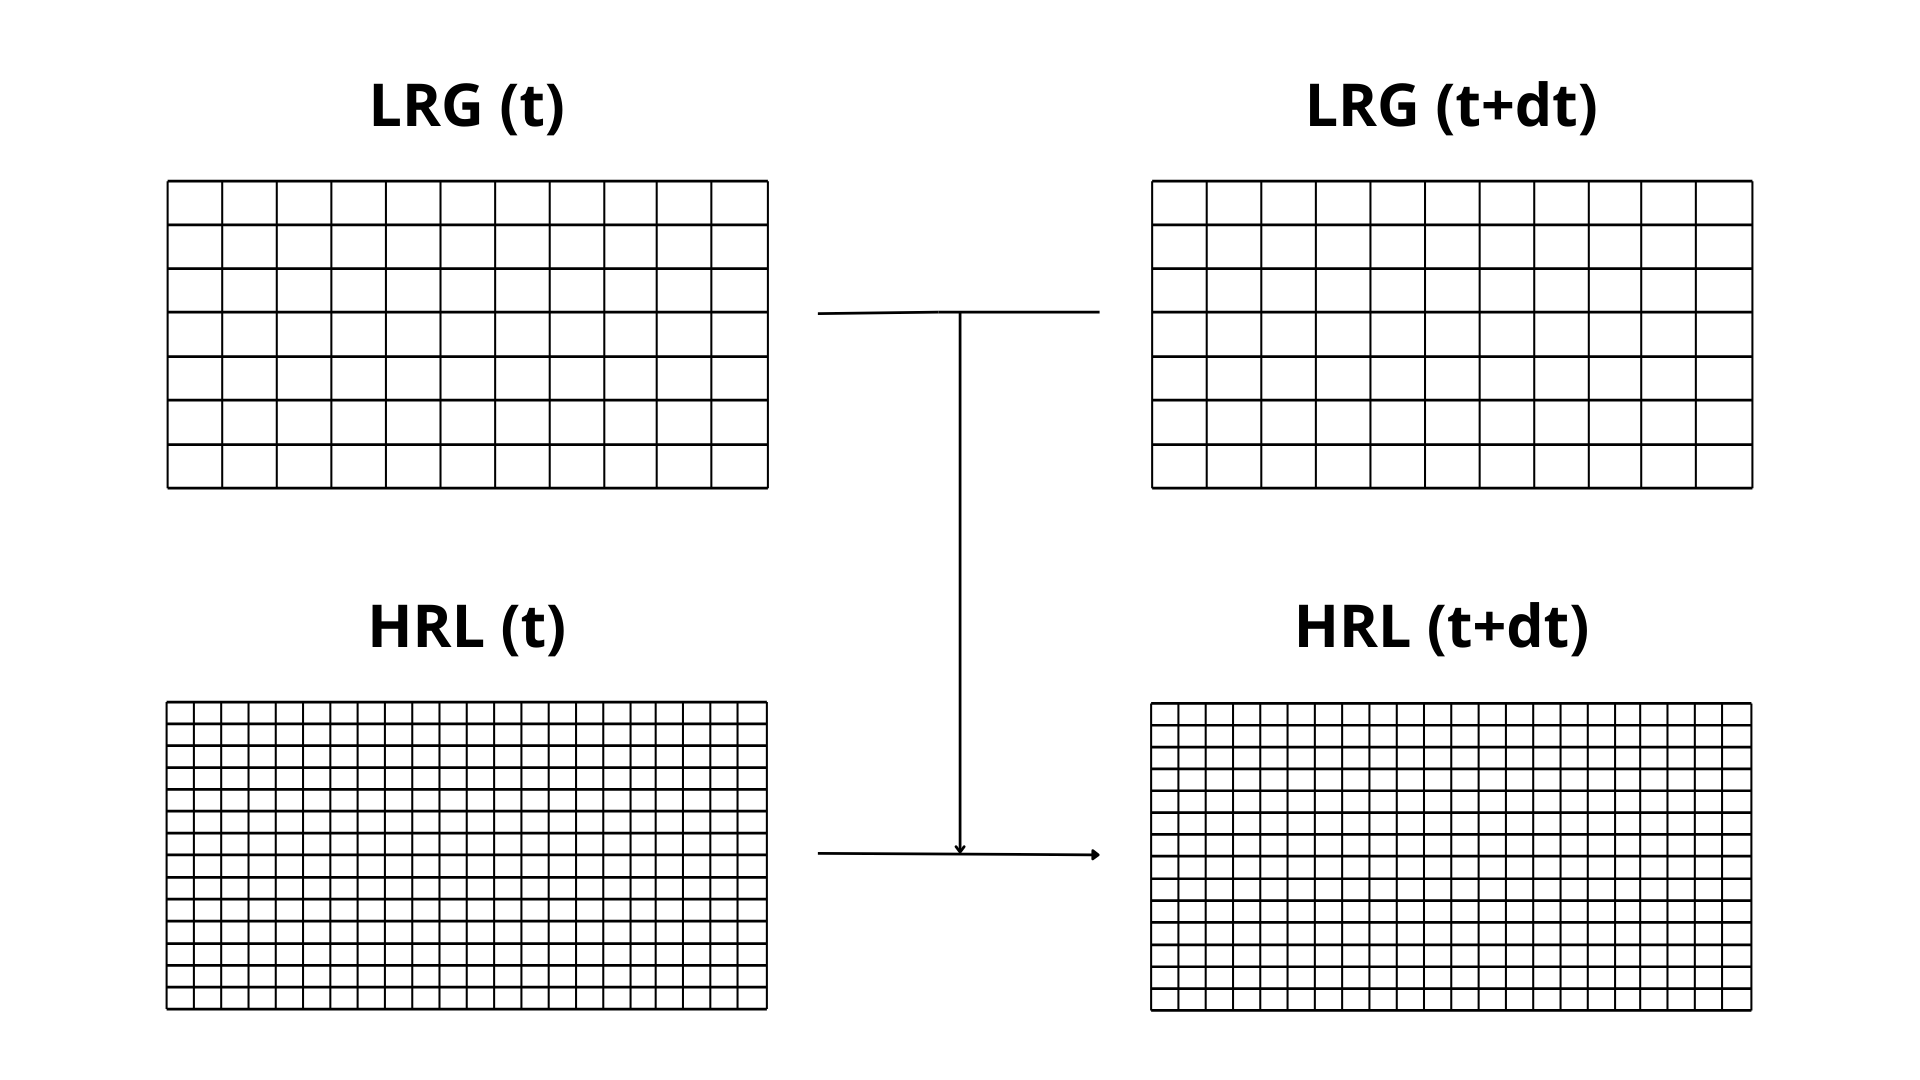
\includegraphics[width=0.8\textwidth]{media/model3.png}
\caption{Architecture of Model 3: Forecast and Downscaling}
\label{fig}
\end{figure}

The objective of this model is to test whether having a broader system state at both time t and time t+dt (the predicted time) with lower resolution can yield better results for the local high-resolution domain at time t+dt. This model involves both forecasting and downscaling steps.

\subsection{Model 4: Rollout or Autoregressive}

\begin{figure}[ht]
\centering
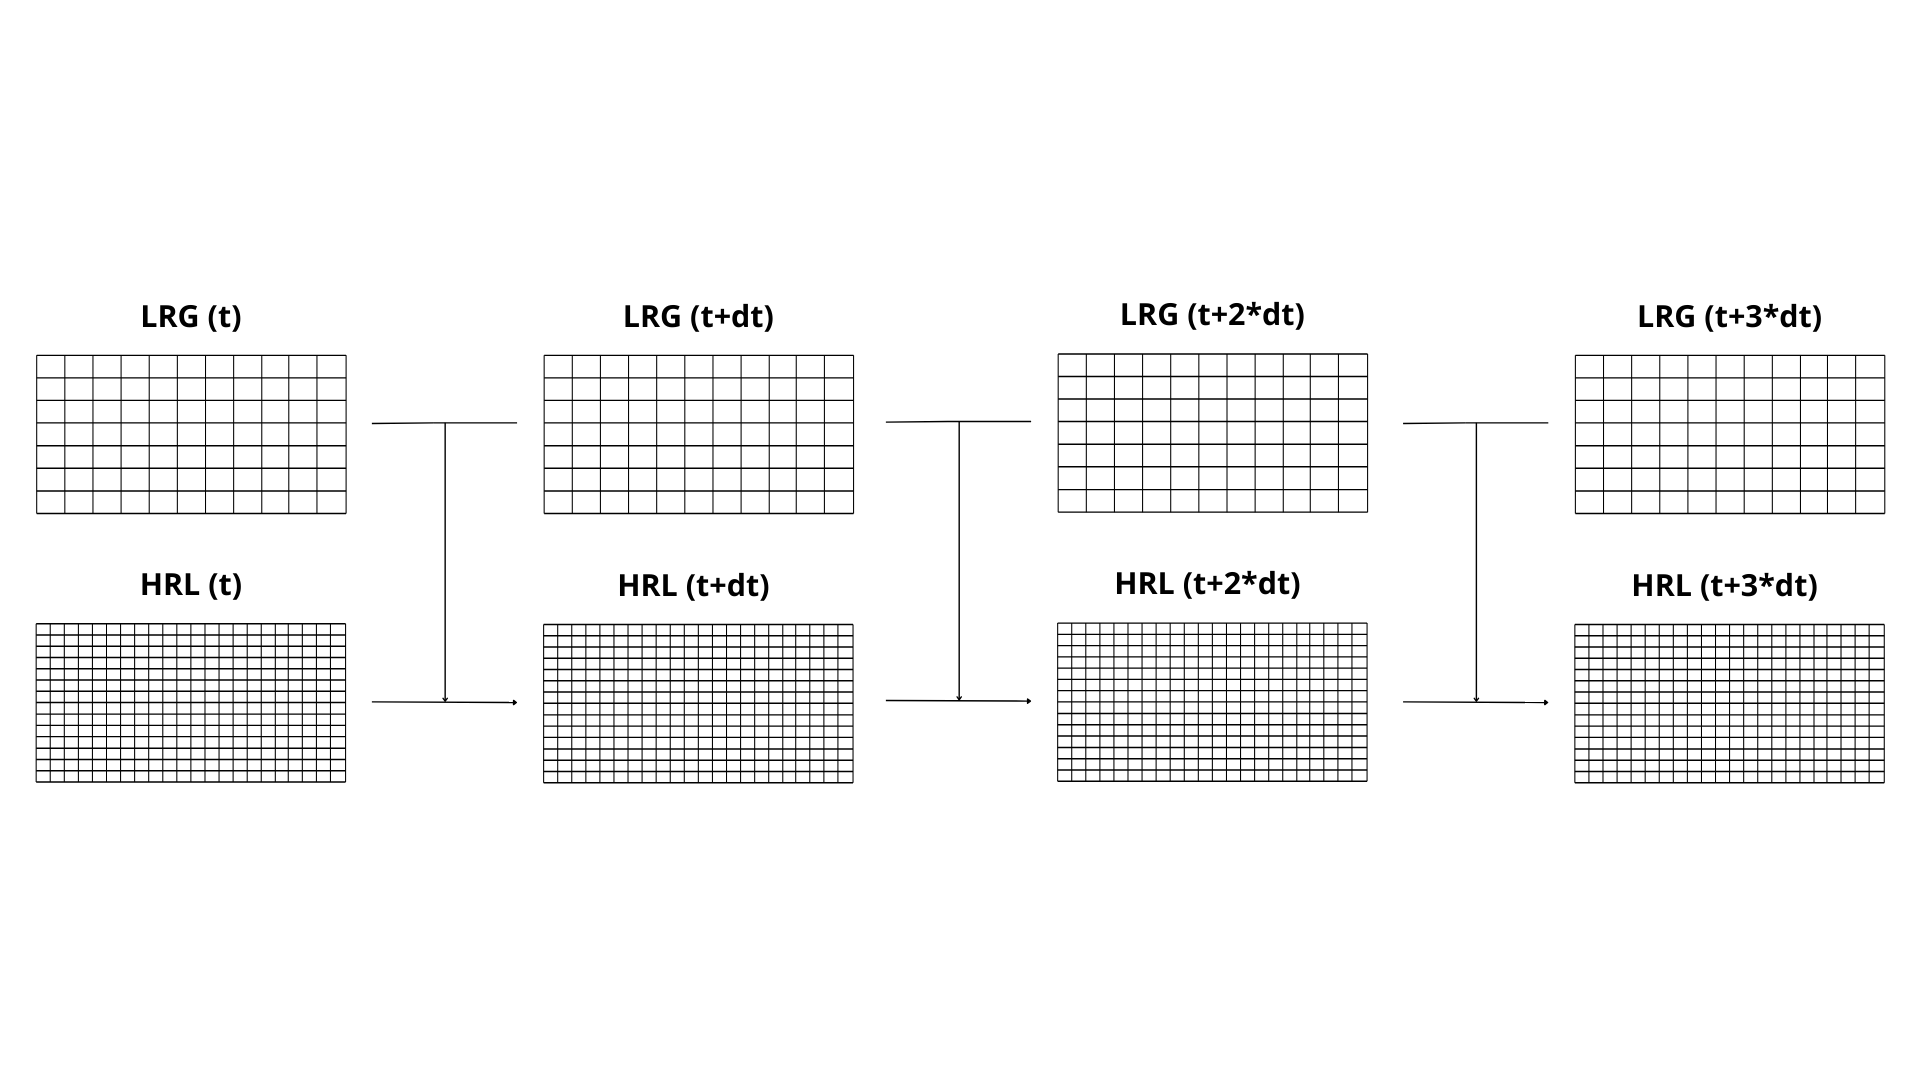
\includegraphics[width=0.9\textwidth]{media/model4.png}
\caption{Architecture of Model 4: Rollout}
\label{fig}
\end{figure}

The output from the previous iteration becomes the new input. The goal is to test the model's ability to predict an output at time n without significant error accumulation.
\newpage